%% 
%% Copyright 2007-2020 Elsevier Ltd
%% 
%% This file is part of the 'Elsarticle Bundle'.
%% ---------------------------------------------
%% 
%% It may be distributed under the conditions of the LaTeX Project Public
%% License, either version 1.2 of this license or (at your option) any
%% later version.  The latest version of this license is in
%%    http://www.latex-project.org/lppl.txt
%% and version 1.2 or later is part of all distributions of LaTeX
%% version 1999/12/01 or later.
%% 
%% The list of all files belonging to the 'Elsarticle Bundle' is
%% given in the file `manifest.txt'.
%% 
%% Template article for Elsevier's document class `elsarticle'
%% with harvard style bibliographic references

%\documentclass[preprint,12pt,authoryear]{elsarticle}

%% Use the option review to obtain double line spacing
%% \documentclass[authoryear,preprint,review,12pt]{elsarticle}

%% Use the options 1p,twocolumn; 3p; 3p,twocolumn; 5p; or 5p,twocolumn
%% for a journal layout:
%% \documentclass[final,1p,times,authoryear]{elsarticle}
%% \documentclass[final,1p,times,twocolumn,authoryear]{elsarticle}
%% \documentclass[final,3p,times,authoryear]{elsarticle}
%% \documentclass[final,3p,times,twocolumn,authoryear]{elsarticle}
%% \documentclass[final,5p,times,authoryear]{elsarticle}
 \documentclass[final,5p,times,twocolumn,authoryear]{elsarticle}

%% For including figures, graphicx.sty has been loaded in
%% elsarticle.cls. If you prefer to use the old commands
%% please give \usepackage{epsfig}

%% The amssymb package provides various useful mathematical symbols
\usepackage{amssymb}
\usepackage{lipsum}
%% The amsthm package provides extended theorem environments
%% \usepackage{amsthm}

%% The lineno packages adds line numbers. Start line numbering with
%% \begin{linenumbers}, end it with \end{linenumbers}. Or switch it on
%% for the whole article with \linenumbers.
%% \usepackage{lineno}

%% You might want to define your own abbreviated commands for common used terms, e.g.:
\newcommand{\kms}{km\,s$^{-1}$}

\journal{}


\begin{document}

\begin{frontmatter}

%% Title, authors and addresses

%% use the tnoteref command within \title for footnotes;
%% use the tnotetext command for theassociated footnote;
%% use the fnref command within \author or \affiliation for footnotes;
%% use the fntext command for theassociated footnote;
%% use the corref command within \author for corresponding author footnotes;
%% use the cortext command for theassociated footnote;
%% use the ead command for the email address,
%% and the form \ead[url] for the home page:
%% \title{Title\tnoteref{label1}}
%% \tnotetext[label1]{}
%% \author{Name\corref{cor1}\fnref{label2}}
%% \ead{email address}
%% \ead[url]{home page}
%% \fntext[label2]{}
%% \cortext[cor1]{}
%% \affiliation{organization={},
%%            addressline={}, 
%%            city={},
%%            postcode={}, 
%%            state={},
%%            country={}}
%% \fntext[label3]{}

\title{Varroa Mites Causing Colony Collapse Disorder}

%% use optional labels to link authors explicitly to addresses:
%% \author[label1,label2]{}
%% \affiliation[label1]{organization={},
%%             addressline={},
%%             city={},
%%             postcode={},
%%             state={},
%%             country={}}
%%
%% \affiliation[label2]{organization={},
%%             addressline={},
%%             city={},
%%             postcode={},
%%             state={},
%%             country={}}

\author[first]{Julia Almeida, Kimberly Ortiz}
\affiliation[first]{organization={The Institute for Computing in Research},%Department and Organization
            addressline={}, 
            city={},
            postcode={}, 
            state={},
            country={}}

\begin{abstract}
%% Text of abstract
Colony Collapse Disorder is a disease that causes bee colonies to rapidly die. The disease kills adult worker bees over the course of 3-4 years. This threat is caused by mites, viruses, parasites, pesticides, and pollution. While there is no current intervention or treatment, this project models colony collapse and explores CRISPR and the DNA sequence of varroa mites as a possible solution to the varroa virus, also known as Deformed Wing Virus. The model simulates the spread of the disease in a colony throughout the summer time. Using python, the project includes an infection model and a graph of the infection over time. We also designed CRISPR guide RNAs to target the viral genome.

\end{abstract}

%%Graphical abstract
%\begin{graphicalabstract}
%\includegraphics{grabs}
%\end{graphicalabstract}

%%Research highlights
%\begin{highlights}
%\item Research highlight 1
%\item Research highlight 2
%\end{highlights}

\begin{keyword}
%% keywords here, in the form: keyword \sep keyword, up to a maximum of 6 keywords 
Varroa mites \sep RNA \sep CRISPR \sep Colony Collapse

%% PACS codes here, in the form: \PACS code \sep code

%% MSC codes here, in the form: \MSC code \sep code
%% or \MSC[2008] code \sep code (2000 is the default)

\end{keyword}


\end{frontmatter}

%\tableofcontents

%% \linenumbers

%% main text

\section{Introduction}
\label{introduction}

The main objective of this project is to demonstrate why honey bee colonies began declining. In recent years high annual losses of honey bee colonies were reported. These losses were attributed to Colony Collapse Disorder. This decline appears to be happening due to several reasons including pathogens, nutrition, beekeeping management, environment, etc. While there’s a big combination of disturbing stressors, pathogens appear to be the highest threat towards honey bees. Especially the Varroa destructor mite, which are tiny red brown external parasites of honey bees. They mainly feed and reproduce on larvae. Therefore this causes the bees' development to be malformed. This should be a concern for all of us due to the fact that a third of our food production depends on bees. As Einstein stated, “If the bee disappeared off the surface of the globe, the man would have only four years of life left. No more bees, no more pollination, no more plants, no more animals, no more man.” 


\section{Background}
\label{Background}

	Over the last sixteen years the number of cases of Colony Collapse Disorder (CDD) have increased substantially. Colony Collapse Disorder is an anomaly that occurs when the majority of worker bees leave behind a hive with no known reason. They leave behind the queen, food, and remaining immature bees. The overall sector for bee health within a colony has had a constant average rate of 28.7\% since 2006-2007. During the winter of 2014-2015 this rate dropped to 23.1\%. As many as 50\% of all affected colonies projected this behavior with no apparent causes. Hives can’t sustain themselves without worker bees and eventually die.  
        Colony losses have been linked to Varroa destructor mites. Varroa mites are a modern honey bee plague that originates from Asia. They attack honey bees directly and indirectly. The mites damage bees directly by attaching and sucking their blood. They affect them indirectly because, like mosquitos, Varroa mites transmit a variety of pathogenic viruses such as Deformed Wing Virus (DWV). This virus has two stages of life: Phorectic and Reproductive Stages. During the first stage the mites begin attaching to bees while feeding on them. The reproductive stage happens in capped brood cells. Capped brood cells are cells that bees cover with a thin film of beeswax to stop evaporation. Female mites lay eggs around 10-12 times on the drone brood. The Varroa mites infestation can build up within 3-4 years. It’s difficult to detect it right away. However colonies with low infestation show general symptoms including; impaired flight performance, lower rate of returning to colony, and reducing their lifespan.

\begin{figure}
  \centering
  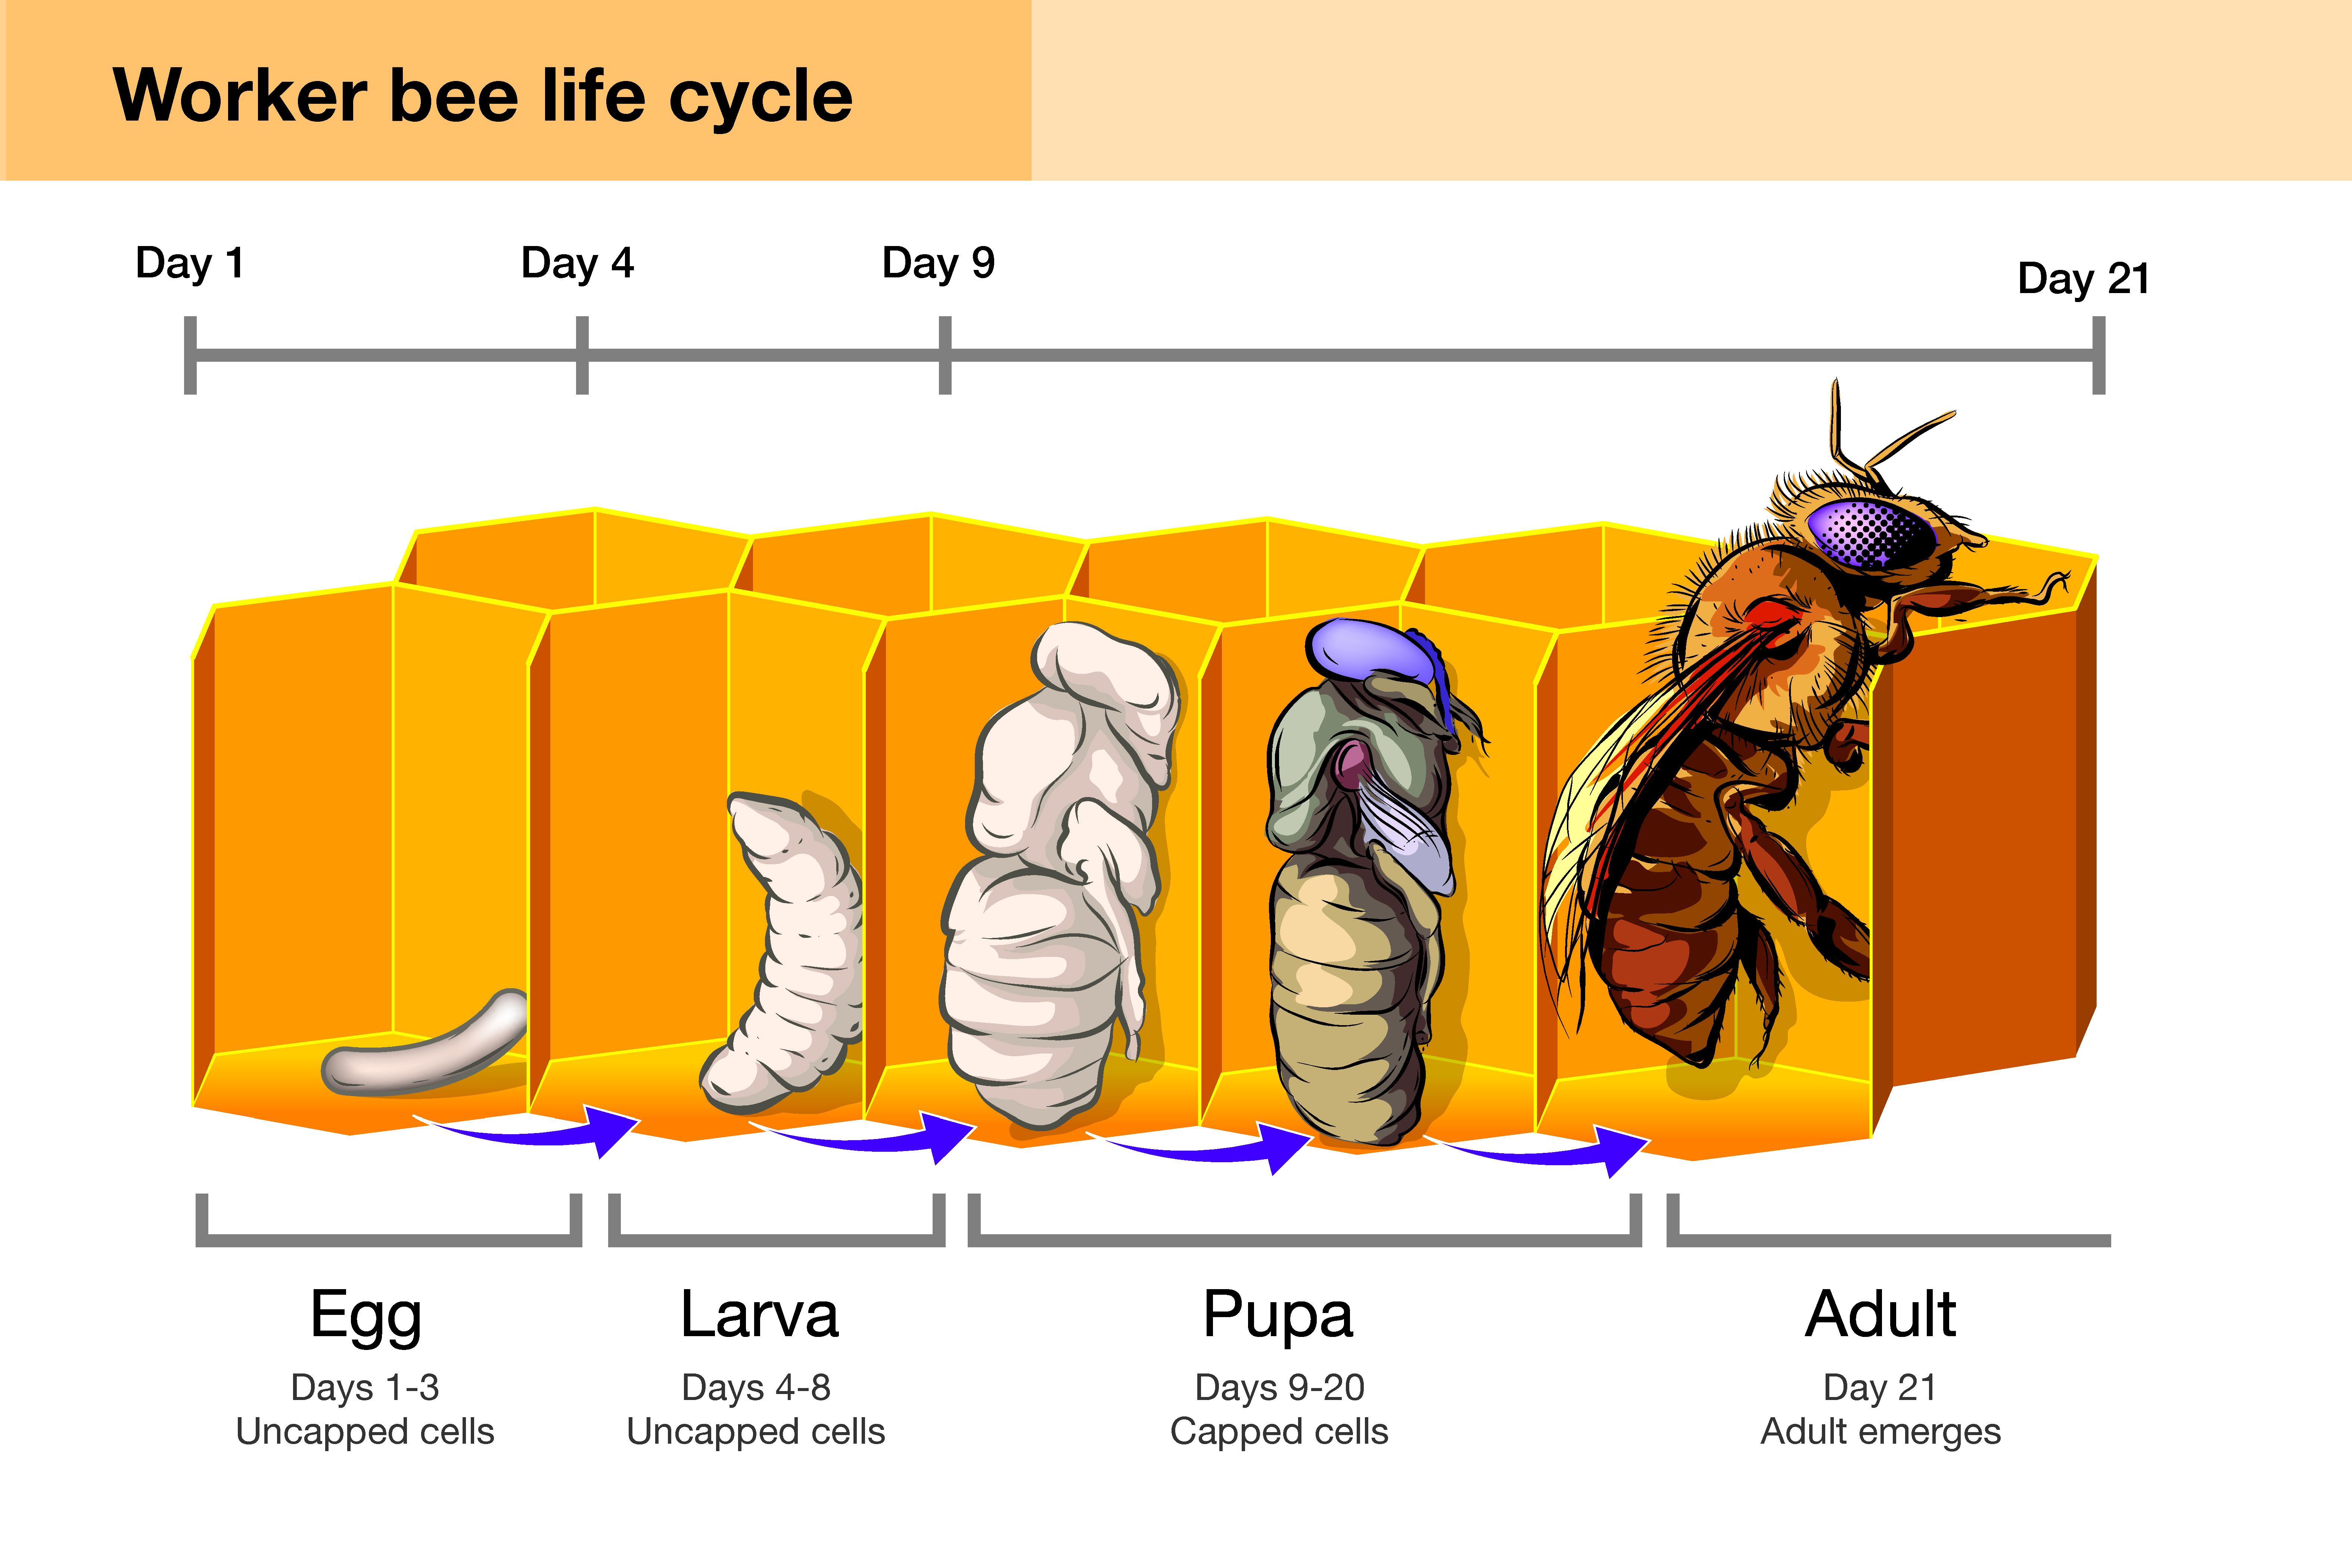
\includegraphics[width=0.4\textwidth, angle=360f]{beecycle.jpg}
  
  Life Cycle of Working Bees
\end{figure}
        
The queen is primarily responsible for the overall genetics of the colony. The queen produces worker bees who are her daughters which then influence the performance of the traits by implementing new activities. The population of a beehive depends on the seasons of the year. In this case we’re only focusing on the summer season, more specifically from April-October. Brood production is at the highest level during this season. There are two types of broods: the Drone Brood and the Worker Brood. You can distinguish these by the way they look, the Drone Brood are large fluffy cells while the Worker Brood are orange capped cells.

Both models demonstrate the bee colonies collapse once infected. Given that treatments only slow progression, we looked at other ways to prevent colony collapse. A method we implemented was CRISPR which is a tool that is used to edit genomes by cutting DNA. CRISPR can correct genetic defects, and treat and prevent spread of disease. In this case, we will use CRISPR to target genes in the viral genome to break them up and kill the virus. We’ll be looking at the genetic sequence of the Varroa virus.


\section{Methods}
\label{Methods}
To simulate the effect of the varroa mites on bee colonies, we created multiple graphs and other visuals. Our first graph (figure 1)  demonstrates the number of infected bees over time based on research that bee scientists have done. Initially, very few bees are infected through the months of April, May, and June. Then the number of infected bees doubles in July and August. In September, the numbers slowly start decreasing. The main part of the simulation is a grid that models infection using mesa and agent based modeling in python. The model shows yellow circles representing bees, and smaller brown circles representing mites. The mites attach to the bees and then infect them, once a bee is infected it is able to infect other bees as well and likely infect the bees with virus. The bees that turn blue are the ones that have been infected for over ten days. 
The goal with CRISPR was to break down the genes in the RNA to attack the virus so it can’t make the proteins it needs. We created a python program to extract the parts of the virus genome that code for proteins so we can target them using CRISPR. We downloaded the single stranded RNA virus (NC\_004830.2) from the National Center for Biotechnology Information (NCBI). We replaced nucleotides that were not A, C, G, or T with N. We found the coordinates for the sequence that codes for the virus proteins in the graphical view at NCBI. We used those coordinates in our python program to get sequences from these regions from the virus genome. Then we put these regions into ChopChop to find guide RNA candidates with good matches to the virus genome but without matches to the bee genome. Using the CHOPCHOP website, we were able to find guide RNA sequences. These will be used with a CRISPR Cas9 subtype that can cut single stranded RNA.

\begin{figure}
  \centering
  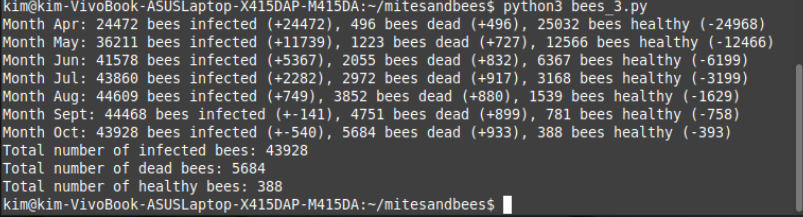
\includegraphics[width=0.5\textwidth, angle=360]{bees_output.png}
  Python output
\end{figure}

\section{Results}
\label{Results}
Figure 1 shows the number of infected, dead, and healthy bees in the range of six months using patterns seen in the literature. The initial number of healthy bees begins with 50,000. This model ends with 391 healthy, 43,920 infected and 5,689 dead bees. As you can see the majority of bees are infected due to the fact that the mites reproduce rapidly and there’s no current treatment. In the second figure we will show a simulation of how a colony infestation looks. 

\begin{figure}
  \centering
  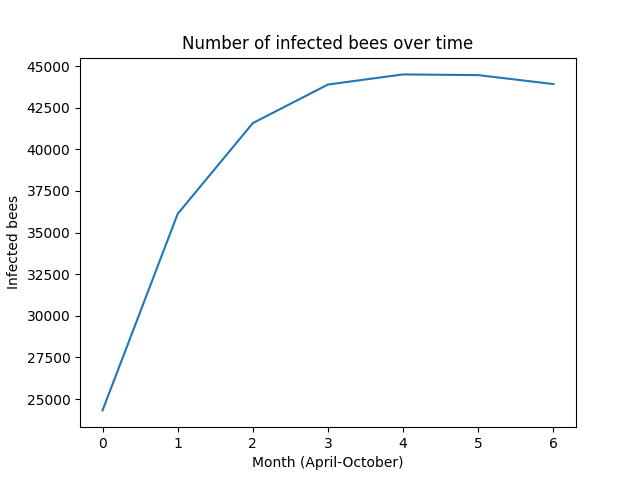
\includegraphics[width=0.4\textwidth, angle=360]{Figure_2.png}
  \caption{Infection Graph}
\end{figure}

This figure demonstrates the simulation of the mites infecting the bees. The yellow dots are the bees, the blue dots are the infected bees that have been infected for more than 10 days and the brown circles are the mites. The mites jump into the yellow dots which then turn blue because they’re infected. If you look closely, the infected bees have a red/brown little dot following them which dictates they’re infected with mites. The infected bees eventually disappear from our simulation because they die or fly away.

\begin{figure}
  \centering
  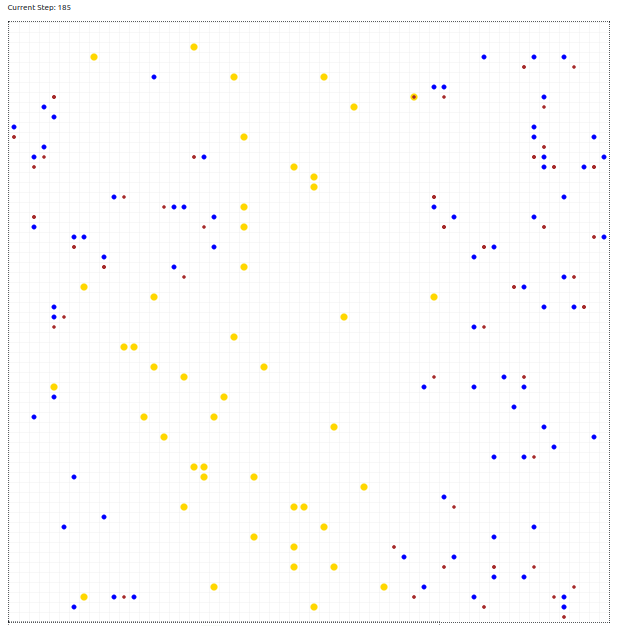
\includegraphics[width=0.4\textwidth, angle=360]{bees_model_pic.png}
  \caption{Agent-Based Model}
\end{figure}

\section*{Discussion}
\label{Discussion}
The increasing heat due to climate change could be a factor in colony collapse disorder because it provides a longer season for bees to forage and possibly infect other colonies. The threat is so serious to bees that the main goal of furthering this project would be to find a solution to eliminate or prevent the disease. Chemical treatments have very little effect on protecting bees. The treatment helped control the varroa mites to some extent but had no effect on the bees that were already infected or the number bees with the virus. During the making of this model, we noticed that the bees were not going to recover. This is when we introduced CRISPR to the project and to allow cutting and destruction of the genome of the varroa viruses. This novel treatment method may help save bee colonies.  

\section{References}
\label{References}
Bee-Health, Seasonality of brood and adult populations (basic bee biology for beekeepers). Bee Health (2019), https://bee-health.extension.org/seasonality-of-brood-and-adult-populations-basic-bee-biology-for-beekeepers/ 

 Bee-Health, Varroa mite reproductive biology. Bee Health (2019), https://bee-health.extension.org/varroa-mite-reproductive-biology/ 

 26. basic agent-based modeling. 26. Basic Agent-Based Modeling - Serious Programming - small courses 0.1.0 documentation, https://markgalassi.codeberg.page/small-courses-html/agent-based-modeling-basics/agent-based-modeling-basics.html 

 Cells, cells and cells.BeeManiacs, https://www.beemaniacs.com/2015/04/18/cells-cells-and-cells/ 

 Chopchop, http://chopchop.cbu.uib.no/results/1690478791663.4148/ 

 Exotic pests. Bee Aware. (n.d.). Retrieved May 2, 2023, from https://beeaware.org.au/archive-pest/varroa-mites/#ad-image-0 

 Maucourt, S., Fortin, F., Robert, C., & Giovenazzo, P. (2020, September 1). Genetic parameters of honey bee colonies traits in a Canadian selection program. Insects. Retrieved May 2, 2023, from https://www.ncbi.nlm.nih.gov/pmc/articles/PMC7564374/  

 R. M. Francis, S. L. Nielsen, P. Kryger, Varroa-virus interaction in collapsing honey bee colonies. PloS one (2013) https://www.ncbi.nlm.nih.gov/pmc/articles/PMC3602523/

 Search: Varroa+virus - NLM. National Center for Biotechnology Information, https://www.ncbi.nlm.nih.gov/search/all/?term=Varroa\%2Bvirus 

Threats to bees. Museum of the Earth. (n.d.). Retrieved May 2, 2023, from https://www.museumoftheearth.org/bees/threats 

Torres, D. J., &amp; Torres, N. A. (2020, September 21). Modeling the influence of mites on honey bee populations. Veterinary sciences. Retrieved May 2, 2023, from https://www.ncbi.nlm.nih.gov/pmc/articles/PMC7559517/ 

 https://pubmed.ncbi.nlm.nih.gov/34850941/

 https://pubmed.ncbi.nlm.nih.gov/16641291/

 https://www.ncbi.nlm.nih.gov/pmc/articles/PMC5796797/

 https://www.google.com/url?sa=i&url\=https\%3A\%2F\%2Fwww
 .serendipi-bee.ca\%2Fbasics\%2Fintro\%2Flife-cycle\%2F&psig=AOvVaw3NGNF6-hIN58-RbvTQ5SfE&ust\=1691078416505000&source\=images&cd=vf
 e&opi=89978449&ved=0CBIQjhxqFwoTCKiVypSs
 voADFQAAAAAdAAAAABAJ 


 
 
%% The Appendices part is started with the command \appendix;
%% appendix sections are then done as normal sections
\appendix

%% If you have bibdatabase file and want bibtex to generate the
%% bibitems, please use
%%
\bibliographystyle{elsarticle-harv} 
\bibliography{example}

%% else use the following coding to input the bibitems directly in the
%% TeX file.

%%\begin{thebibliography}{00}

%% \bibitem[Author(year)]{label}
%% For example:

%% \bibitem[Aladro et al.(2015)]{Aladro15} Aladro, R., Martín, S., Riquelme, D., et al. 2015, \aas, 579, A101


%%\end{thebibliography}

\end{document}

\endinput
%%
%% End of file `elsarticle-template-harv.tex'.
